%%%%%%%%%%%%%%%%%%%%%
%%%%% PREAMBULE %%%%%
%%%%%%%%%%%%%%%%%%%%%
\documentclass[a4paper,12pt,twoside]{book}
\usepackage{fontspec}

%%%%% Index %%%%%
%\usepackage{index}
%\usepackage{imakeidx}%pour les index, à charger avant hyperref
%\makeindex
%\makeindex[name=lieux, title=Index des noms de lieux]%créer un index des lieux

\usepackage[pdfusetitle, pdfsubject ={Mémoire TNAH}, pdfkeywords={institut national de l'audiovisuel; référentiel; thésaurus; vocabulaire contrôlé; vocabulaire hiérarchique; ontologie; web de données; Wikidata; liens; alignement}]{hyperref}
\usepackage[french]{babel}
\usepackage{morewrites}
\usepackage{tocbibind} %paquet pour mettre index et bib dans la toc

% configurer le document selon les normes de l'école
\usepackage[margin=2.5cm]{geometry}
\usepackage{setspace}
\onehalfspacing
\setlength\parindent{1cm}

\usepackage{lettrine}

%%%%% Dessin %%%%%
%\usepackage{qtree}
% avec un code comme ça pour un arbre de classification
%\Tree[.IP [.NP [.Det \textit{the} ]
%[.N\1 [.N \textit{package} ]]]
%[.I\1 [.I \textsc{3sg.Pres} ]
%[.VP [.V\1 [.V \textit{is} ]
%[.AP [.Deg \textit{really} ]
%[.A\1 [.A \textit{simple} ]
%\qroof{\textit{to use}}.CP ]]]]]]
\usepackage{tikz} %paquet pour dessiner ; à placer avant graphicx
\usepackage{graphicx} %paquet image


\usepackage{caption} %pour que la mention de figure n'apparaisse pas dans les légendes de l'image


%%%%% Bibliographie %%%%%
%\usepackage[backend=biber, sorting=nyt, style=enc, maxbibnames=3]{biblatex}
%\addbibresource{bibliographie/bib.bib}
%\nocite{*}
%\defbibnote{intro}{Cette bibliographie contient toutes les références utilisées pour ce cours} %pour des notes introductives dans le début de la biblio

%%%%% Abréviations %%%%%
\usepackage{acro}
\DeclareAcronym{ina}{short = INA, long = Institut National de l'Audiovisuel}
% appel par \ac{ina}


%%%%% Nouvelles commandes %%%%%
% \newcommand{\reference}[1]{\autoref{#1}: \nameref{#1}}

\newcommand{\chaptertoc}[1]{\chapter*{#1}
	\addcontentsline{toc}{chapter}{#1}
	\markboth{\slshape\MakeUppercase{#1}}{\slshape\MakeUppercase{#1}}}

\newcommand{\titreEntete}[1]{\markboth{\slshape\MakeUppercase{#1}}{}}

%%%%% Nouveaux environnements %%%%%

\author{Maxime Challon - M2 TNAH}
\title{Les référentiels en institutions patrimoniales : évolution des pratiques et repositionnement. L’exemple des référentiels de l’Institut National de l’Audiovisuel.}

%%%%%%%%%%%%%%%%%%%%
%%%%% DOCUMENT %%%%%
%%%%%%%%%%%%%%%%%%%%
\begin{document}	
	\frontmatter
	\begin{titlepage}
		\begin{center}
			
			\bigskip
			
			\begin{large}
				\'ECOLE NATIONALE DES CHARTES
			\end{large}
			\begin{center}\rule{2cm}{0.02cm}\end{center}
			
			\bigskip
			\bigskip
			\bigskip
			\begin{Large}
				\textbf{Maxime Challon}\\
			\end{Large}
			\begin{normalsize} \textit{licencié ès histoire}
			\end{normalsize}
			
			\bigskip
			\bigskip
			\bigskip
			
			\begin{Huge}
				\textbf{Les référentiels en institutions patrimoniales : évolution des pratiques et repositionnement}\\
			\end{Huge}
			\bigskip
			\bigskip
			\begin{LARGE}
				\textbf{L’exemple des référentiels de l’Institut National de l’Audiovisuel}\\
			\end{LARGE}
			
			\bigskip
			\bigskip
			\bigskip
			\begin{large}
			\end{large}
			\vfill
			
			\begin{large}
				Mémoire 
				pour le diplôme de master \\
				\og{} Technologies numériques appliquées à l'histoire \fg{} \\
				\bigskip
				2020
			\end{large}
			
		\end{center}
	\end{titlepage}

\thispagestyle{empty}	
\cleardoublepage
	
		\chapter*{Résumé}
	\titreEntete{Résumé}
\addcontentsline{toc}{chapter}{Résumé}
	\medskip
	Ce mémoire, réalisé pour l'obtention du diplôme de Master 2 \og Technologies numériques appliquées à l'histoire\fg{} de l'École nationale des Chartes, retrace l'évolution des pratiques documentaires sur les référentiels en institution patrimoniale à travers l'étude des référentiels de l'\ac{ina} et leurs alignements. Cette étude de l'évolution des formes et des structures des référentiels est liée à l'évolution de la place de ces référentiels au sein des systèmes documentaires, ainsi qu'aux besoins qui leur sont liés.\\
	
	\textbf{Mots-clés~:} institut national de l'audiovisuel; référentiel; thésaurus; vocabulaire contrôlé; vocabulaire hiérarchique; ontologie; web de données; Wikidata; liens; alignement.
	
	\textbf{Informations bibliographiques~:} Maxime Challon, \textit{Les référentiels en institutions patrimoniales : évolution des pratiques et repositionnement. L’exemple des référentiels de l’Institut National de l’Audiovisuel.}, mémoire de master \og{}Technologies numériques appliquées à l'histoire\fg{}, dir. Gautier Poupeau, École nationale des chartes, 2020.
	
		\chapter*{Remerciements}
	\titreEntete{Remerciements}
	\addcontentsline{toc}{chapter}{Remerciements}
	
	\lettrine{M}es remerciements vont tout d'abord à Gautier \textsc{Poupeau}, mon maître de stage, qui m'a accueilli, guidé, conseillé et intégré à son équipe malgré le travail à distance imposé par le contexte actuel. Je souhaite également remercier Axel \textsc{Roche-Dioré} pour ses explications et son soutien dans la réalisation technique de mon stage.\\
	
	J'adresse aussi mes remerciements aux membres du pôle \og Ingénierie de la Donnée\fg{}, Lauryne \textsc{Lemosquet}, Otmane \textsc{Elabboubi} et Akli \textsc{Abdi} pour le temps qu'ils m'ont accordé. \\
	
	Que soit également remercié l'ensemble du département \og Architecture et Innovation\fg{} de l'\ac{ina} pour l'accompagnement fourni tout au long de mon stage, notamment Stanislas \textsc{de Maigret} et Matthieu \textsc{Boricaud} pour le déploiement de l'application, et Olivio \textsc{Ségura} pour la présentation des archives de l'\ac{ina}.
	
	\chaptertoc{Liste des abréviations}
	\printacronyms[heading=none]
	
		\chapter*{\label{introduction_generale}Introduction}
	\titreEntete{Introduction}
\addcontentsline{toc}{chapter}{Introduction}

\begin{citationLongue}
	Toutefois pour ne laisser cette quantité infinie ne la définissant point, [et] aussi pour ne jetter les curieux hors d'espérance et pouvoir acco[m]plir [et] venir à bout de cette belle entreprise, il me semble qu'il est à propos de faire comme les Médecins, qui ordonnent la quantité des drogues suivant la qualité d'icelles, [et] de dire que l'on ne peut manquer de recueillir tous ceux qui auront les qualitez [et] conditions requises pour estre mis dans une Bibliotheque.\footcite[p.41-42]{naude_advis_1627}
\end{citationLongue}


\lettrine{E}n 1627, \nP{Gabriel}{Naudé} compare le médecin au bibliothécaire, semblables par leur nécessité d'ordonner pour sélectionner, de classer pour retrouver, au milieu d'une masse d'objets. Cet ordonnancement, ce classement, passent pas une hiérarchisation de leur connaissance ou de leurs outils, dans le but de faciliter la recherche d'un médicament ou d'un livre pour l'utilisateur final. Cependant, plusieurs siècles plus tard, la hiérarchisation de la connaissance, ayant pour but de référencer une instance de la vie réelle, ne fonctionne plus: l'utilisateur ne part plus que très rarement d'un terme de la hiérarchie pour trouver son document; il utilise le plus souvent un mot ou un concept qui le renverront vers une liste de résultats correspondant à sa requête. Alors, la notion de graphe prend le dessus sur celle de hiérarchie.\\

La notion évoquée de \og quantité infinie \fg{} est aujourd'hui d'autant plus valable avec le web et l'explosion des quantités de données produites et stockées: avec cette mort de la notion de ressource, et par conséquent de celle de référentiel, la donnée structurée est implantée, peut être exploitée à la fois par une machine et par une personne, et est divisible et modulable à l'infini.\\

Cette transition de la ressource à la donnée, des référentiels hiérarchiques aux référentiels en graphe, est observable à l'\ac{ina}. Créé en 1975 suite au démantèlement en sept sociétés de l'\ac{ortf} par la loi du 07 août 1974, l'\ac{ina} est désigné comme un \ac{epic} et \og chargé de la conservation des archives, des recherches de créations audiovisuelles et de la formation professionnelle\fg{}\footcite[art.3]{noauthor_loi_1974}. À ces missions est ajouté à partir de 1992 le dépôt légal de la télévision, de la radio, de la télévision satellite, par câble et numérique. Cette massification continue de documents et de données nécessite un classement et un référencement efficace des collections, ce qui a conduit à la création de plusieurs référentiels dans l'Institut.\\

Face à la croissance de l'utilisation du numérique, à l'accroissement des collections et des données à l'\ac{ina} depuis les numérisations des collections au début des années 2000, aux nouveaux besoins exprimés par les professionnels et le public, une refonte du système documentaire est mise en place à la \ac{dsi} au sein du département \og Architecture et Innovation\fg{}: les données et leurs métadonnées sont extraites des anciens silos de conservation, puis transformées et migrées dans un nouveau système d'information centralisé. Ainsi, les référentiels, descripteurs de chaque document, identificateurs de personnes ou d'instances des collections, subissent également ce traitement pour les uniformiser et permettre une homogénéisation et une meilleure valorisation des données de l'\ac{ina}.\\

Cette migration massive permet d'observer l'évolution des pratiques documentaires de référencement et de description de ces dernières décennies, suivant la même évolution que l'ensemble du milieu bibliothéconomique en France, ainsi que les changements de structure des référentiels utilisés. La diversité de formes et de structures des référentiels montre que ces derniers sont considérés seulement comme des outils à disposition du documentaliste pour décrire ses fonds; périphériques et éclatés, ils ne permettent pas une centralisation uniforme des données de l'\ac{ina}.\\

Le projet du \textit{Lac de données}, débuté en 2014, a pour but de centraliser l'ensemble des données de l'\ac{ina}, les référentiels prenant alors une place centrale dans le nouveau système d'information. Ce projet s'inscrit dans l'évolution des besoins, tant chez les documentalistes que chez les utilisateurs, avec une utilisation désormais massive du web par tous les publics - chercheurs, professionnels des médias, jeunesse, \dots - pour la recherche et la consultation de contenus. Cette éditorialisation croissante et indispensable nécessite de nombreuses données de référence, par lesquelles les contenus sont cherchables et trouvables.\\

Ce mémoire offre une réflexion sur ces évolutions des pratiques et des usages des référentiels à l'\ac{ina}, et plus généralement dans une institution patrimoniale. Au-delà de ces évolutions sensibles, c'est le positionnement du référentiel au sein des systèmes documentaires qu'il est nécessaire d'interroger, de manière à faire face aux nouveaux enjeux et aux nouveaux besoins exprimés ces dernières années: d'un rôle périphérique, pensé comme un outil, le référentiel devient désormais un pivot autour duquel les données documentaires se raccrochent.\\

Mon stage, débuté en mai 2020 et terminé fin août 2020, à la \ac{dsi} de l'\ac{ina}, m'a permis d'intégrr le département \og Architecture et Innovation\fg{} de \nP{Gautier}{Poupeau}, et plus particulièrement le pôle \og Ingénierie de la Donnée\fg{} dirigé par \nP{Axel}{Roche-Dioré}, afin d'effectuer une réflexion sur les méthodes d'alignement de plusieurs référentiels, et de mettre en œuvre ces méthodes. Les échanges avec mes collègues du pôle \og Ingénierie de la Donnée\fg{} et les professionnels de la documentation de la \ac{ddcol} et de la \ac{dj} m'ont permis de naviguer dans les référentiels, d'observer leurs différences, leurs structures, de comprendre les besoins qui leurs étaient associés ainsi que les difficultés impliquées par chaque référentiel dans l'opération d'alignement en vue de leur migration vers le \textit{Lac de données}. Plusieurs missions m'ont ainsi été confiées:
\begin{itemize}
	\item Extraire les fonctions et les occupations de personnes physiques depuis les notes qualité en texte libre du référentiel des personnes physiques et morales de la \ac{ddcol}, puis aligner ces fonctions extraites avec un thésaurus de noms communs propre à la \ac{ddcol}
	\item Aligner les personnes physiques de la \ac{ddcol} avec les entités correspondantes de \href{https://www.wikidata.org/}{Wikidata}
	\item Aligner les fictions et les séries conservées à l'\ac{ina} avec \href{https://www.wikidata.org/}{Wikidata} de manière à récupérer également l'identifiant \ac{isan}
	\item Aligner les référentiels de personnes physiques de la \ac{dj} et de la \ac{ddcol}, puis développer une interface de vérification et de complétion des alignements réalisés automatiquement
\end{itemize}
\bigskip

Ce mémoire retrace l'évolution des usages et des pratiques documentaires concernant les référentiels dans les institutions patrimoniales, en s'appuyant sur l'exemple des référentiels de l'\ac{ina}. Dans un premier temps, dans une période allant jusqu'au début des années 2000, les référentiels sont uniquement considérés comme des fournisseurs de clés entre les données de manière à les contrôler plus facilement. Puis, jusqu'au milieu des années 2010, le web et le web de données permettent une mise en commun des référentiels qui se retrouvent alors liés entre eux. Enfin, depuis le milieu des années 2010, les référentiels sont placés au centre des systèmes d'information: ils sont devenus les pivots des systèmes documentaires.


\thispagestyle{empty}
\cleardoublepage
	
	\mainmatter
	
	\part{\label{controler}CONTRÔLER. A la recherche de clés (années 1960 – fin des années 1990)}
	
	\chapter{\label{I-A}Le référentiel comme clé}
	\titreEntete{Le référentiel comme clé}
	\chapter{\label{I-B}L'arbre, un vocabulaire contrôlé hiérarchique}
	\titreEntete{L'arbre, un vocabulaire contrôlé hiérarchique}
	\chapter{\label{I-C}Les référentiels à l’INA}
	\titreEntete{Les référentiels à l’INA}
	
	\part{\label{relier}RELIER. Vers le partage de référentiels communs (début des années 2000 – milieu des années 2010)}
	
	\chapter{\label{II-A}Le web de données: une exposition commune des référentiels}
	\titreEntete{Le web de données: une exposition commune des référentiels}
	\chapter{\label{II-B}Partager des structurations similaires de jeux de données par les classes et les propriétés : les ontologies, grammaires communes mais spécifiques}
	\titreEntete{Les ontologies, grammaires communes mais spécifiques}
	\chapter{\label{II-C}Relier ses données à Wikidata}
	\titreEntete{Relier ses données à Wikidata}
	
	\part{\label{centraliser}CENTRALISER. Le référentiel, clé de voûte et pivot (depuis le milieu des années 2010)}	
	
	\chapter{\label{III-A}Les labyrinthes comme réseaux de données et de liens}
	\titreEntete{Les labyrinthes comme réseaux de données et de liens}
	\chapter{\label{III-B}Le Lac de données de l’INA : le référentiel au centre du modèle}
	\titreEntete{Le référentiel au centre du modèle}
	\chapter{\label{III-C}Centraliser les référentiels de l’INA dans le Lac de données: l'exemple de l'alignement de deux référentiels de personnes physiques}
	\titreEntete{Aligner deux référentiels de personnes physiques}

	\chaptertoc{Conclusion}
\titreEntete{Conclusion}

%historique de struct ref: arbre au laby et modele reseau

%changement des usages et des besoins...

%... qui produit changement place ref
	
	\appendix
	\part*{Annexes}	
	\addcontentsline{toc}{part}{Annexes}
	\setcounter{chapter}{0}

\chapter{\label{annexe_index_schoepflin}Les index de la Renaissance, termes contrôlés et classification alphabétique (les index de l'\textit{Alsatia Illustrata} de \nP{Jean-Daniel}{Schoepflin})}
\titreEntete{Annexe \thechapter}

\begin{figure}[!h]
	\centering
	\begin{minipage}[c]{.46\linewidth}
		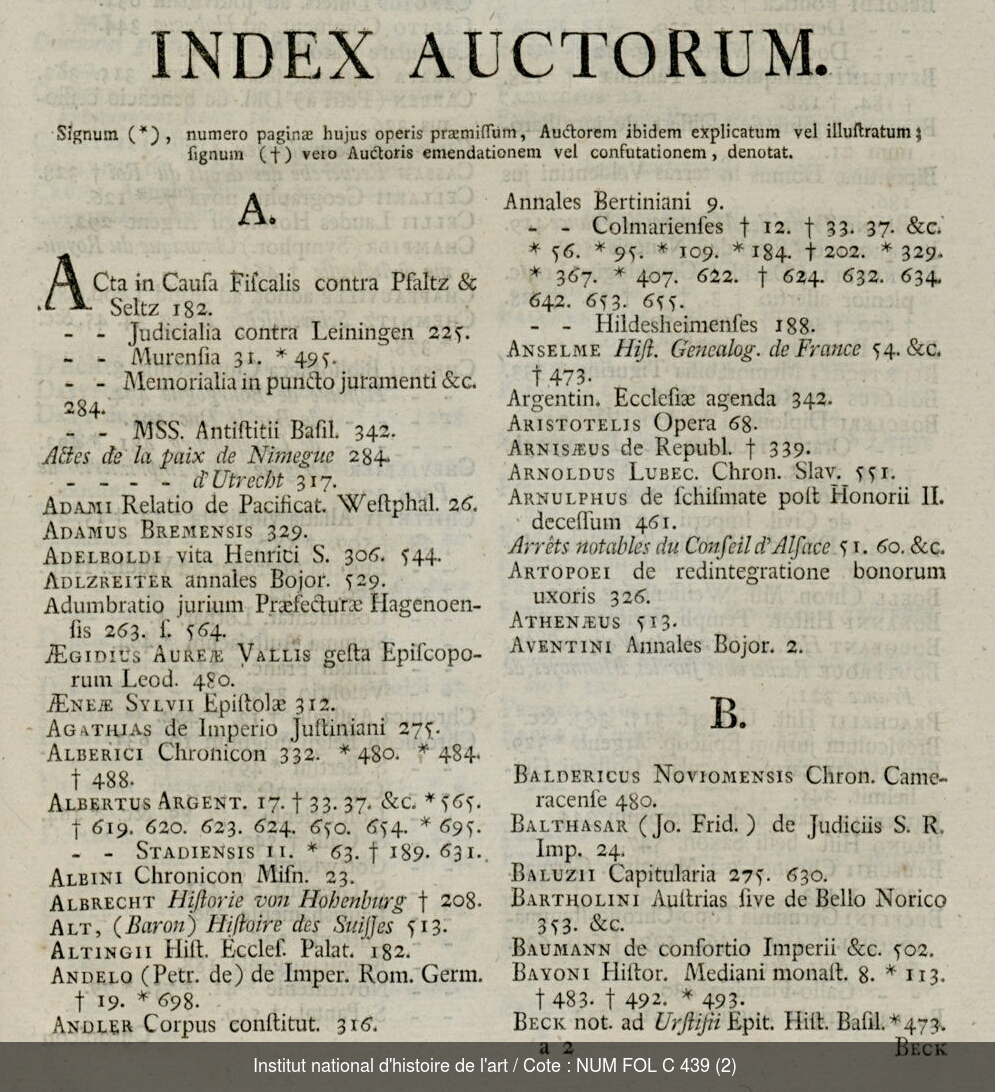
\includegraphics[width=6cm]{images/index_auctorum_alsatia.jpg}
		\caption{Index auctorum}
	\end{minipage} \hfill
	\begin{minipage}[c]{.46\linewidth}
		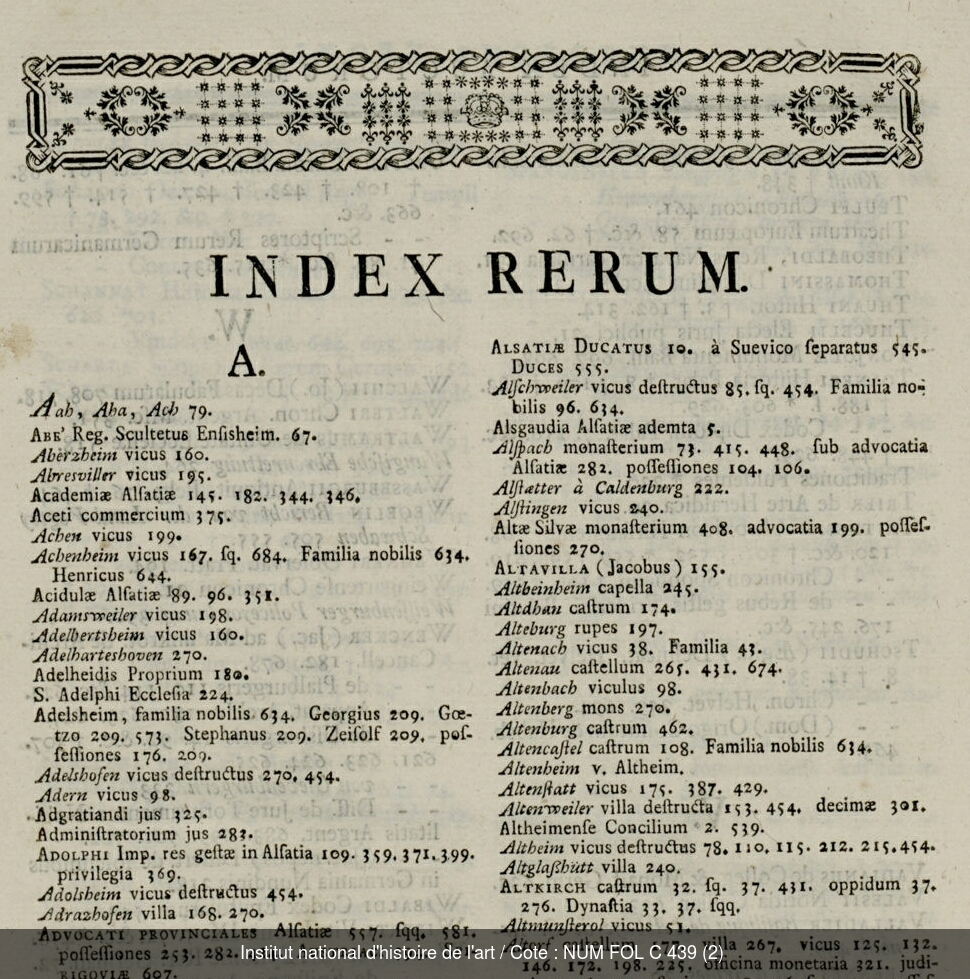
\includegraphics[width=6cm]{images/index_rerum_alsatia.jpg}
		\caption{Index rerum}
	\end{minipage} 
	\medskip
	Extraits des deux index de l'œuvre de \nP{Jean-Daniel}{Schoepflin} [Source: \url{http://bibliotheque-numerique.inha.fr/idurl/1/12532}, p.804 et 813]
\end{figure}

\chapter{\label{annexe_types_interop}Les différents types d'interopérabilité}
\titreEntete{Annexe \thechapter}

\begin{figure}[!h]
	\centering
	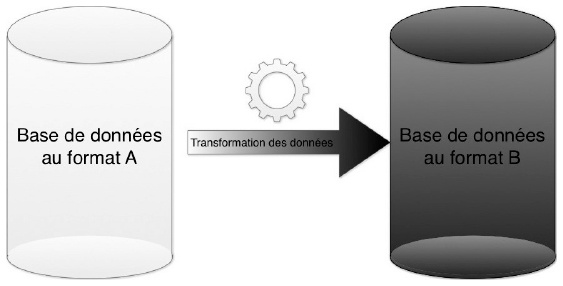
\includegraphics[width=12cm]{images/interop_conversion_copie.jpeg}
	\medskip
	\caption[L'interopérabilité par conversion et copie]{L'interopérabilité par conversion et copie [Source: \cite{bermes_2_2013}]}
\end{figure}

\begin{figure}[!h]
	\centering
	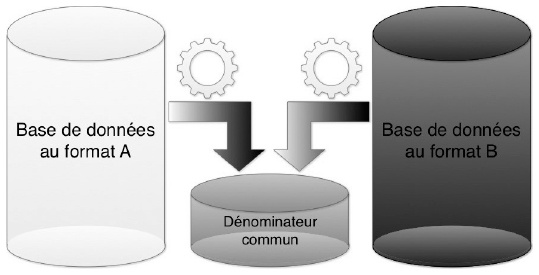
\includegraphics[width=12cm]{images/interop_denom_commun.jpeg}
	\medskip
	\caption[L'interopérabilité par le plus petit dénominateur commun]{L'interopérabilité par le plus petit dénominateur commun [Source: \cite{bermes_2_2013}]}
\end{figure}
	
	\backmatter
	
	
%bibliographie ici dans les normes de l'école
%\printbibliography[title= Bibliographie sélective, prenote=intro]%postnote est aussi possible
%\printbibliography[heading=subbibliography, keyword={semantique}, title={Sémantique}]%biblio sélective pour un mot clé donné

% index à mettre ici si index	
%	\printindex
%\printindex[lieux]

	\listoffigures

	\tableofcontents
	
\end{document}